\documentclass[letterpaper]{article}
% FinFM @ AAAI-27 (benchmark track, non-archival). Official AAAI-27 style, anonymous
% submission. The lines marked "fixed" come from the author kit and must stay as they are.
% The body is shared with the ACL 2027 draft: sections, numbers and figures are read from
% ../latex_acl2027 so the two versions cannot drift apart.
\usepackage[submission]{aaai2027}
\usepackage[hyphens]{url} % fixed
\usepackage{graphicx} % fixed
\urlstyle{rm} % fixed
\def\UrlFont{\rm} % fixed
\usepackage{natbib} % fixed, without options
\usepackage{caption} % fixed, without options
\frenchspacing % fixed
\setlength{\pdfpagewidth}{8.5in} % fixed
\setlength{\pdfpageheight}{11in} % fixed
\usepackage{amsmath,amssymb,booktabs,array,listings}
\usepackage{tikz}
\usetikzlibrary{arrows.meta,positioning,fit,backgrounds,calc,shadows,shapes.geometric,3d,shadows.blur,fadings,shadings}
\definecolor{finblue}{HTML}{2A78D6}
\definecolor{finorange}{HTML}{EB6834}
\definecolor{fingray}{HTML}{52514E}
\definecolor{finaqua}{HTML}{1BAF7A}
\definecolor{finmagenta}{HTML}{C2408B}
% Small pictograms for the figures, drawn in TikZ (no icon font needed). Use as
% \pic[draw=white, line width=0.55pt] at (x,y) {fin doc}; size about 0.3 cm.
\tikzset{
  fin doc/.pic={
    \draw[pic actions, fill=none, line join=round] (-0.10,-0.14) -- (-0.10,0.14) -- (0.04,0.14)
      -- (0.10,0.08) -- (0.10,-0.14) -- cycle;
    \draw[pic actions, fill=none] (0.04,0.14) -- (0.04,0.08) -- (0.10,0.08);
    \draw[pic actions, fill=none, line width=0.4pt] (-0.055,0.03) -- (0.055,0.03)
      (-0.055,-0.025) -- (0.055,-0.025) (-0.055,-0.08) -- (0.03,-0.08);},
  fin check/.pic={
    \draw[pic actions, fill=none] (0,0) circle (0.13);
    \draw[pic actions, fill=none, line width=0.75pt, line cap=round, line join=round]
      (-0.065,0.0) -- (-0.018,-0.05) -- (0.07,0.055);},
  fin loop/.pic={
    \draw[pic actions, fill=none, line width=0.7pt, -{Stealth[length=2.4pt, width=2.8pt]}]
      (0.13,0.0) arc[start angle=0, end angle=285, radius=0.12];},
  fin plug/.pic={
    \draw[pic actions, fill=none, rounded corners=0.6pt] (-0.09,-0.02) rectangle (0.09,0.07);
    \draw[pic actions, fill=none, line cap=round] (-0.045,0.07) -- (-0.045,0.14) (0.045,0.07) -- (0.045,0.14);
    \draw[pic actions, fill=none, line cap=round] (0,-0.02) -- (0,-0.14);},
  fin robot/.pic={
    \draw[pic actions, fill=none, rounded corners=1pt] (-0.12,-0.10) rectangle (0.12,0.08);
    \fill[pic actions, draw=none] (-0.05,-0.005) circle (0.022) (0.05,-0.005) circle (0.022);
    \draw[pic actions, fill=none, line cap=round] (0,0.08) -- (0,0.13);
    \fill[pic actions, draw=none] (0,0.145) circle (0.022);},
  fin gauge/.pic={
    \draw[pic actions, fill=none] (-0.13,-0.05) arc[start angle=180, end angle=0, radius=0.13];
    \draw[pic actions, fill=none, line width=0.7pt, line cap=round] (0,-0.05) -- (0.07,0.04);
    \fill[pic actions, draw=none] (0,-0.05) circle (0.025);},
  fin lock/.pic={
    \draw[pic actions, fill=none, rounded corners=0.8pt] (-0.10,-0.13) rectangle (0.10,0.02);
    \draw[pic actions, fill=none] (-0.06,0.02) -- (-0.06,0.07) arc[start angle=180, end angle=0,
      radius=0.06] -- (0.06,0.02);
    \fill[pic actions, draw=none] (0,-0.055) circle (0.022);},
  fin chart/.pic={
    \fill[pic actions, draw=none] (-0.11,-0.12) rectangle (-0.05,-0.02)
      (-0.03,-0.12) rectangle (0.03,0.06) (0.05,-0.12) rectangle (0.11,0.12);},
  fin code/.pic={
    \draw[pic actions, fill=none, line cap=round, line join=round, line width=0.65pt]
      (-0.06,0.08) -- (-0.13,0) -- (-0.06,-0.08) (0.06,0.08) -- (0.13,0) -- (0.06,-0.08);
    \draw[pic actions, fill=none, line cap=round, line width=0.5pt] (0.025,0.11) -- (-0.025,-0.11);},
  fin search/.pic={
    \draw[pic actions, fill=none, line width=0.6pt] (-0.025,0.035) circle (0.085);
    \draw[pic actions, fill=none, line width=0.9pt, line cap=round] (0.04,-0.03) -- (0.11,-0.11);},
  fin feed/.pic={
    \fill[pic actions, draw=none] (-0.085,-0.085) circle (0.028);
    \draw[pic actions, fill=none, line width=0.6pt, line cap=round]
      (-0.085,0.005) arc[start angle=90, end angle=0, radius=0.09]
      (-0.085,0.075) arc[start angle=90, end angle=0, radius=0.16];},
  fin link/.pic={
    \draw[pic actions, fill=none, line width=0.6pt, rounded corners=1.6pt, rotate=45]
      (-0.13,-0.04) rectangle (0.0,0.04) (-0.0,-0.04) rectangle (0.13,0.04);},
  fin sigma/.pic={
    \draw[pic actions, fill=none, line width=0.7pt, line cap=round, line join=round]
      (0.085,0.11) -- (-0.085,0.11) -- (0.02,0.0) -- (-0.085,-0.11) -- (0.085,-0.11);},
  fin db/.pic={
    \draw[pic actions, fill=none, line width=0.6pt] (0,0.085) ellipse (0.1 and 0.035);
    \draw[pic actions, fill=none, line width=0.6pt] (-0.1,0.085) -- (-0.1,-0.085)
      arc[start angle=180, end angle=360, x radius=0.1, y radius=0.035] -- (0.1,0.085);
    \draw[pic actions, fill=none, line width=0.5pt] (-0.1,0.0)
      arc[start angle=180, end angle=360, x radius=0.1, y radius=0.035];},
  fin braces/.pic={
    \draw[pic actions, fill=none, line width=0.65pt, rounded corners=0.9pt, line cap=round]
      (-0.025,0.12) -- (-0.065,0.12) -- (-0.065,0.03) -- (-0.115,0) -- (-0.065,-0.03)
      -- (-0.065,-0.12) -- (-0.025,-0.12)
      (0.025,0.12) -- (0.065,0.12) -- (0.065,0.03) -- (0.115,0) -- (0.065,-0.03)
      -- (0.065,-0.12) -- (0.025,-0.12);},
  fin term/.pic={
    \draw[pic actions, fill=none, line width=0.55pt, rounded corners=1pt]
      (-0.13,-0.1) rectangle (0.13,0.1);
    \draw[pic actions, fill=none, line width=0.65pt, line cap=round, line join=round]
      (-0.075,0.035) -- (-0.03,0.0) -- (-0.075,-0.035);
    \draw[pic actions, fill=none, line width=0.65pt, line cap=round] (0.0,-0.045) -- (0.07,-0.045);},
  fin person/.pic={
    \fill[pic actions, draw=none] (0,0.055) circle (0.052);
    \fill[pic actions, draw=none] (-0.11,-0.125) arc[start angle=180, end angle=0, radius=0.11]
      -- cycle;},
}

% Generated by make_numbers.py from the library; do not edit by hand.
\newcommand{\NSkills}{131}
\newcommand{\NPlugins}{17}
\newcommand{\NReferenceFiles}{75}
\newcommand{\NScripts}{125}
\newcommand{\NListingTokens}{27,700}
\newcommand{\NFederatedPacks}{92}
\newcommand{\NFederatedSkills}{2,390}
\newcommand{\NLensPacks}{3}
\newcommand{\NLensSkills}{100}
\newcommand{\NKOLProfiles}{40}
\newcommand{\NAlgorithms}{48}
\newcommand{\NAlgorithmTasks}{11}
\newcommand{\NNative}{25}
\newcommand{\NAdapters}{23}
\newcommand{\NOptionalLibraries}{13}
\newcommand{\NGuards}{39}
\newcommand{\NGuardsExported}{32}
\newcommand{\NGuardsPythonOnly}{7}
\newcommand{\NTools}{67}
\newcommand{\NCards}{6}
\newcommand{\NCardFamilies}{3}
\newcommand{\NCauses}{5}
\newcommand{\NMethods}{7}
\newcommand{\NArms}{4}
\newcommand{\NTasks}{34}
\newcommand{\NTaskAlgorithms}{17}
\newcommand{\NDevTasks}{18}
\newcommand{\NDevAlgorithms}{9}
\newcommand{\NHeldTasks}{16}
\newcommand{\NHeldAlgorithms}{8}
\newcommand{\NHeldFamilies}{5}
\newcommand{\NFamilies}{5}
\newcommand{\NSeeds}{3}
\newcommand{\NRows}{128}
\newcommand{\NRowsEFour}{96}
\newcommand{\NEFourTasks}{4}
\newcommand{\NForcedDev}{5}
\newcommand{\NDrawn}{12}
\newcommand{\NDrawnDev}{4}
\newcommand{\NModels}{5}
\newcommand{\NMainEpisodes}{3,360}
\newcommand{\NAblationEpisodes}{1,440}
\newcommand{\NRealEpisodes}{1,120}
\newcommand{\NRealRows}{128}
\newcommand{\NRealSplitRow}{45}
\newcommand{\RealFirst}{31 March 2022}
\newcommand{\RealLast}{3 October 2022}
\newcommand{\RefGapMinVariance}{1.4\times10^{-6}}
\newcommand{\RefGapOther}{2.8\times10^{-14}}
\newcommand{\BudgetAttempts}{3}
\newcommand{\BudgetCalls}{6}
\newcommand{\BudgetTokens}{12,000}
\newcommand{\FitEpisodes}{48}
\newcommand{\FitProposals}{6}
\newcommand{\FitCalls}{600}
\newcommand{\FitTokens}{1,200,000}
\newcommand{\EvolveGenerations}{3}
\newcommand{\EvolveMinibatch}{4}

\graphicspath{{../latex_acl2027/}}
\makeatletter\def\input@path{{../latex_acl2027/}}\makeatother % shared tables
\lstset{basicstyle=\ttfamily\footnotesize,columns=fullflexible,keepspaces=true,
        showstringspaces=false,frame=none,xleftmargin=0pt}
\newcommand{\pending}[1]{{\color{red}[#1]}}
\providecommand{\href}[2]{#2} % aaai2027.bst emits \href; AAAI forbids hyperref
\newcommand{\lib}{\textsc{Fin-RSI}}
\setcounter{secnumdepth}{2}

\title{\lib{}: An Agent-Native Library of Financial Skills, Checks, and Self-Improvement}
\author{Anonymous submission}
\affiliations{}

\begin{document}
\maketitle

\begin{abstract}
Financial research code fails silently: a program that applies stock splits twice, or
trades on the closing price it reads, still runs and still returns a backtest. We present
\lib{}, an agent-native Python library that puts three things behind interfaces a language-model
agent can call. \emph{Skills} are \NSkills{} dated skill documents, \NAlgorithms{} algorithms
and \NCards{} rule cards. \emph{Checks} are \NGuards{} guards, including property checks that
need no expected output. \emph{Self-improvement} is \NMethods{} methods, from self-debugging
and reflection to playbook learning and prompt evolution, behind one
\texttt{fit}/\texttt{solve}/\texttt{state} interface with metered, equal budgets. With the
library comes a suite of \NTasks{} financial programming tasks. Each task has an independent
reference and a hidden grader that no method sees, and the suite is split by algorithm into
development and held-out sets. The evaluation protocol separates the contributions of skills,
checks and self-improvement. \pending{One sentence of results once the experiments are
complete.} The library, the tasks and the protocol will be released.

\end{abstract}

\begin{figure*}[t]
\centering
% Figure 1: the library at a glance. Information comes in on the left, an agent is composed in
% the middle (the user's model, one self-improvement method, any checks, skills and investor
% templates) and the library is used from the right. Badges and labels are counts from the code
% on 2026-11-05: macros from numbers.tex where one exists, otherwise noted here (8 adapters,
% 4 discovery sources, 9 collectors in fin_skills.data and fin_skills.collect; 14 bridged
% libraries in fin_skills.bridges). Needs the TikZ libraries 3d, shadows.blur, fadings, shadings.
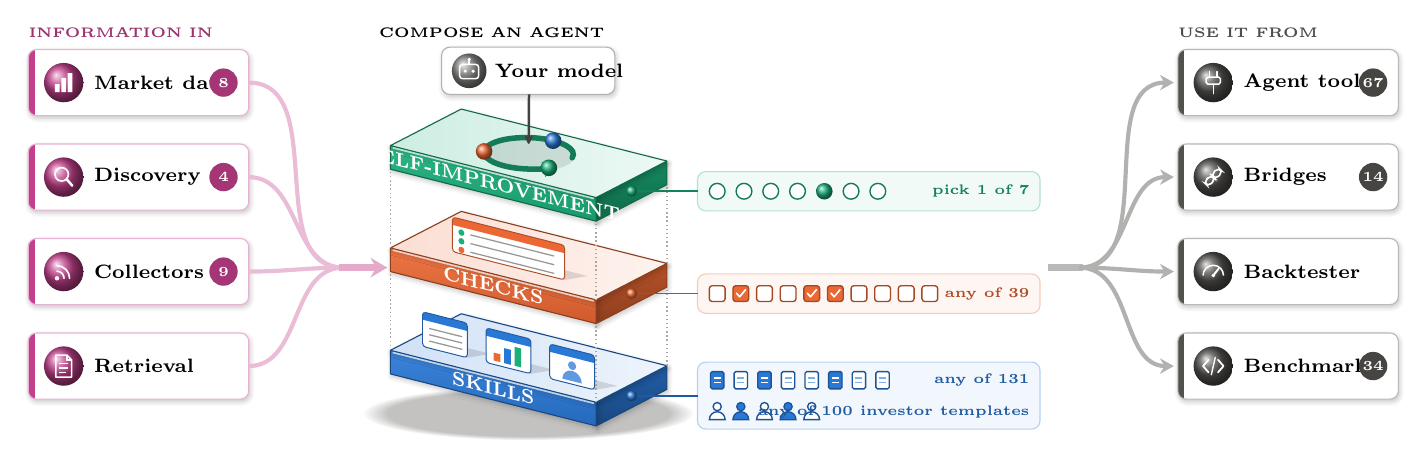
\begin{tikzpicture}[
  font=\scriptsize,
  >={Stealth[length=4pt, width=3.8pt, round]},
  head/.style={font=\tiny\bfseries, anchor=south west, inner sep=0pt},
  ball/.style={circle, shading=ball, ball color=#1, inner sep=0pt, minimum size=9pt},
  ball/.default=finblue,
  iso/.style={x={(0.95cm,-0.24cm)}, y={(0.62cm,0.32cm)}, z={(0cm,1cm)}},
  shade/.style={blur shadow={shadow blur steps=6, shadow xshift=0.45pt, shadow yshift=-0.9pt,
                             shadow opacity=24}},
  badge/.style={circle, fill=#1, text=white, font=\tiny\bfseries, inner sep=0pt,
                minimum size=0.36cm},
  pick/.style={font=\tiny\bfseries, text=#1!75!black, anchor=east, inner sep=0pt},
]
% ================================================================== helpers
% \tile{x}{y centre}{w}{colour}{icon}{label}{badge}: a card with an accent bar, an icon and a count.
\newcommand{\tile}[7]{%
  \path[fill=white, rounded corners=3pt, shade] (#1,{#2+0.42}) rectangle ({#1+#3},{#2-0.42});
  \begin{scope}
    \clip[rounded corners=3pt] (#1,{#2+0.42}) rectangle ({#1+#3},{#2-0.42});
    \fill[#4] (#1,{#2+0.42}) rectangle ({#1+0.08},{#2-0.42});
  \end{scope}
  \draw[#4!40, rounded corners=3pt, line width=0.4pt] (#1,{#2+0.42}) rectangle ({#1+#3},{#2-0.42});
  \node[ball=#4, minimum size=0.5cm] at ({#1+0.45},#2) {};
  \pic[draw=white, fill=white, line width=0.55pt] at ({#1+0.45},#2) {#5};
  \node[anchor=west, font=\scriptsize\bfseries, inner sep=0pt] at ({#1+0.83},#2) {#6};
  \if\relax\detokenize{#7}\relax\else
    \node[badge=#4!85!black] at ({#1+#3-0.32},#2) {#7};\fi}
% \track{y bottom}{y top}{colour}: the tinted strip that holds one layer's choices.
\newcommand{\track}[3]{%
  \path[fill=#3!6, draw=#3!35, line width=0.4pt, rounded corners=3pt] (8.5,#1) rectangle (12.85,#2);}
\def\sW{2.75}\def\sD{1.45}\def\sT{0.3}\def\pitch{1.3}
% \slab{z}{colour}{label}: a shaded slab with its label printed on the front face.
\newcommand{\slab}[3]{%
  \begin{scope}[iso]
    \shade[top color=#2!78!black, bottom color=#2!60!black]
      (\sW,0,#1) -- (\sW,\sD,#1) -- (\sW,\sD,{#1+\sT}) -- (\sW,0,{#1+\sT}) -- cycle;
    \shade[top color=#2!92, bottom color=#2!88!black]
      (0,0,#1) -- (\sW,0,#1) -- (\sW,0,{#1+\sT}) -- (0,0,{#1+\sT}) -- cycle;
    \shade[left color=#2!22, right color=#2!8]
      (0,0,{#1+\sT}) -- (\sW,0,{#1+\sT}) -- (\sW,\sD,{#1+\sT}) -- (0,\sD,{#1+\sT}) -- cycle;
    \draw[#2!60!black, line width=0.4pt, line join=round]
      (0,0,#1) -- (\sW,0,#1) -- (\sW,\sD,#1) -- (\sW,\sD,{#1+\sT}) -- (0,\sD,{#1+\sT})
      -- (0,0,{#1+\sT}) -- cycle (0,0,{#1+\sT}) -- (\sW,0,{#1+\sT}) -- (\sW,\sD,{#1+\sT})
      (\sW,0,{#1+\sT}) -- (\sW,0,#1);
    \draw[white, opacity=0.7, line width=0.6pt] (0.03,0,{#1+\sT-0.02}) -- (\sW-0.03,0,{#1+\sT-0.02});
    \begin{scope}[canvas is xz plane at y=0]
      \node[transform shape, text=white, font=\scriptsize\bfseries] at (\sW/2, {#1+\sT/2}) {#3};
    \end{scope}
  \end{scope}}
% \stand{x}{y}{z}{w}{h}{colour}{content}: a card standing on a top face, shadow cast behind.
\newcommand{\stand}[7]{%
  \begin{scope}[iso]
    \begin{scope}[canvas is xy plane at z=#3]
      \fill[black, opacity=0.12] (#1, #2) -- ({#1+#4}, #2) -- ({#1+#4+0.14}, {#2+0.26})
        -- ({#1+0.14}, {#2+0.26}) -- cycle;
    \end{scope}
    \begin{scope}[canvas is xz plane at y=#2, shift={(#1, #3)}]
      \fill[white, rounded corners=1.2pt] (0,0) rectangle (#4, #5);
      \begin{scope}
        \clip[rounded corners=1.2pt] (0,0) rectangle (#4, #5);
        \fill[#6] (0, #5-0.1) rectangle (#4, #5);
      \end{scope}
      \draw[#6!75!black, line width=0.35pt, rounded corners=1.2pt] (0,0) rectangle (#4, #5);
      #7
    \end{scope}
  \end{scope}}

% ================================================================== left: information in
\node[head, text=finmagenta!80!black] at (0, 5.22) {INFORMATION IN};
\tile{0}{4.65}{2.8}{finmagenta}{fin chart}{Market data}{8}
\tile{0}{3.45}{2.8}{finmagenta}{fin search}{Discovery}{4}
\tile{0}{2.25}{2.8}{finmagenta}{fin feed}{Collectors}{9}
\tile{0}{1.05}{2.8}{finmagenta}{fin doc}{Retrieval}{}
\foreach \y in {4.65, 3.45, 2.25, 1.05}
  \draw[line width=1.5pt, finmagenta!35] (2.8, \y) to[out=0, in=180] (4.0, 2.3);
\draw[-{Stealth[length=6pt, width=7pt]}, line width=2.4pt, finmagenta!45] (3.95, 2.3) -- (4.56, 2.3);

% ================================================================== middle: compose an agent
\node[head] at (4.45, 5.22) {COMPOSE AN AGENT};
\begin{scope}[shift={(4.6, 0.95)}]
\fill[fingray, opacity=0.35, path fading=circle with fuzzy edge 15 percent]
  (1.75, -0.5) ellipse (2.1cm and 0.34cm);
\slab{0}{finblue}{SKILLS}
\stand{0.22}{0.32}{\sT}{0.6}{0.44}{finblue}{%
  \foreach \yy in {0.25, 0.17, 0.09} \draw[fingray!60, line width=0.45pt] (0.09,\yy) -- (0.53,\yy);}
\stand{1.07}{0.32}{\sT}{0.6}{0.44}{finblue}{%
  \fill[finorange] (0.1,0.05) rectangle (0.19,0.15); \fill[finblue] (0.24,0.05) rectangle (0.33,0.24);
  \fill[finaqua] (0.38,0.05) rectangle (0.47,0.29);}
\stand{1.92}{0.32}{\sT}{0.6}{0.44}{finblue}{%
  \fill[finblue!75] (0.3,0.235) circle (0.055);
  \fill[finblue!75] (0.17,0.04) arc[start angle=180, end angle=0, radius=0.13] -- cycle;}
\slab{\pitch}{finorange}{CHECKS}
\stand{0.62}{0.32}{{\pitch+\sT}}{1.5}{0.44}{finorange}{%
  \foreach \yy/\c in {0.27/finaqua, 0.16/finaqua, 0.05/finorange} {
    \fill[\c] (0.12,\yy) circle (0.04); \draw[fingray!60, line width=0.45pt] (0.24,\yy) -- (1.36,\yy);}}
\slab{2*\pitch}{finaqua}{SELF-IMPROVEMENT}
\begin{scope}[iso]
  \begin{scope}[canvas is xy plane at z={2*\pitch+\sT}]
    \fill[black, opacity=0.1] (\sW/2+0.05, \sD/2-0.06) circle (0.5);
    \draw[finaqua!70!black, line width=2pt, line cap=round, -{Stealth[length=4.5pt, width=5.5pt]}]
      ({\sW/2+0.5*cos(20)}, {\sD/2+0.5*sin(20)}) arc[start angle=20, end angle=340, radius=0.5];
  \end{scope}
  \foreach \a/\c in {90/finblue, 210/finorange, 330/finaqua}
    \node[ball=\c, minimum size=6pt] at ({\sW/2+0.5*cos(\a)}, {\sD/2+0.5*sin(\a)}, {2*\pitch+\sT}) {};
  \foreach \u/\v in {0/0, \sW/0, \sW/\sD}
    \draw[fingray!50, densely dotted, line width=0.5pt]
      (\u, \v, \sT) -- (\u, \v, \pitch) (\u, \v, {\pitch+\sT}) -- (\u, \v, {2*\pitch});
  \foreach \k in {0, 1, 2} \coordinate (r\k) at (\sW, \sD/2, {\k*\pitch+\sT/2});
  \coordinate (topc) at (\sW/2, \sD/2, {2*\pitch+\sT});
\end{scope}
\end{scope}

% the user's model drives the stack
\path[fill=white, rounded corners=3pt, shade] (5.25, 5.1) rectangle (7.45, 4.5);
\draw[fingray!45, rounded corners=3pt, line width=0.4pt] (5.25, 5.1) rectangle (7.45, 4.5);
\node[ball=fingray!70, minimum size=0.44cm] (rob) at (5.6, 4.8) {};
\pic[draw=white, fill=white, line width=0.55pt] at (rob) {fin robot};
\node[anchor=west, font=\scriptsize\bfseries, inner sep=0pt] at (5.92, 4.8) {Your model};
\draw[->, line width=0.9pt, fingray!80!black] (6.36, 4.5) -- ($(topc) + (0, 0.12)$);

% each layer's choices: filled marks are one agent
\track{3.02}{3.52}{finaqua}
\track{1.72}{2.22}{finorange}
\track{0.25}{1.1}{finblue}
\foreach \k/\col in {0/finblue, 1/finorange, 2/finaqua} {
  \draw[\col!75!black, line width=0.5pt] (r\k) -- (r\k -| 8.5, 0);
  \node[ball=\col, minimum size=4pt] at (r\k) {};}
% self-improvement: pick one (radio)
\foreach \i in {0,...,6} {
  \ifnum\i=4 \node[ball=finaqua, minimum size=0.21cm] at ({8.75+0.34*\i}, 3.27) {};
  \else \draw[finaqua!70!black, fill=white, line width=0.5pt] ({8.75+0.34*\i}, 3.27) circle (0.1);\fi}
\node[pick=finaqua] at (12.72, 3.27) {pick 1 of \NMethods{}};
% checks: pick any (boxes)
\foreach \i in {0,...,9} {
  \def\cx{8.75+0.3*\i}
  \ifnum\i=1 \def\on{1}\else\ifnum\i=4 \def\on{1}\else\ifnum\i=5 \def\on{1}\else\def\on{0}\fi\fi\fi
  \ifnum\on=1
    \draw[finorange!70!black, fill=finorange, line width=0.5pt, rounded corners=1pt]
      ({\cx-0.1}, 1.87) rectangle ({\cx+0.1}, 2.07);
    \draw[white, line width=0.6pt, line cap=round, line join=round]
      ({\cx-0.055}, 1.975) -- ({\cx-0.015}, 1.93) -- ({\cx+0.06}, 2.02);
  \else
    \draw[finorange!70!black, fill=white, line width=0.5pt, rounded corners=1pt]
      ({\cx-0.1}, 1.87) rectangle ({\cx+0.1}, 2.07);\fi}
\node[pick=finorange] at (12.72, 1.97) {any of \NGuards{}};
% skills: pick any (documents) and investor templates (people)
\foreach \i in {0,...,7} {
  \def\cx{8.75+0.3*\i}
  \ifnum\i=0 \def\on{1}\else\ifnum\i=2 \def\on{1}\else\ifnum\i=5 \def\on{1}\else\def\on{0}\fi\fi\fi
  \ifnum\on=1 \def\fc{finblue}\def\lc{white}\else \def\fc{white}\def\lc{finblue!60}\fi
  \draw[finblue!70!black, fill=\fc, line width=0.5pt, rounded corners=0.6pt]
    ({\cx-0.085}, 0.76) rectangle ({\cx+0.085}, 0.98);
  \draw[\lc, line width=0.45pt] ({\cx-0.045}, 0.90) -- ({\cx+0.045}, 0.90)
    ({\cx-0.045}, 0.84) -- ({\cx+0.045}, 0.84);}
\node[pick=finblue] at (12.72, 0.87) {any of \NSkills{}};
\foreach \i in {0,...,4} {
  \def\cx{8.75+0.3*\i}
  \ifnum\i=1 \def\fc{finblue}\else\ifnum\i=3 \def\fc{finblue}\else\def\fc{white}\fi\fi
  \draw[finblue!70!black, fill=\fc, line width=0.5pt] (\cx, 0.535) circle (0.052);
  \draw[finblue!70!black, fill=\fc, line width=0.5pt]
    ({\cx-0.1}, 0.37) arc[start angle=180, end angle=0, radius=0.1] -- cycle;}
\node[pick=finblue] at (12.72, 0.46) {any of \NLensSkills{} investor templates};

% ================================================================== right: use it from
\node[head, text=fingray!95!black] at (14.6, 5.22) {USE IT FROM};
\tile{14.6}{4.65}{2.8}{fingray}{fin plug}{Agent tools}{\NTools{}}
\tile{14.6}{3.45}{2.8}{fingray}{fin link}{Bridges}{14}
\tile{14.6}{2.25}{2.8}{fingray}{fin gauge}{Backtester}{}
\tile{14.6}{1.05}{2.8}{fingray}{fin code}{Benchmark}{\NTasks{}}
\draw[line width=2.4pt, fingray!40] (12.95, 2.3) -- (13.4, 2.3);
\foreach \y in {4.65, 3.45, 2.25, 1.05}
  \draw[-{Stealth[length=5pt, width=5.5pt]}, line width=1.5pt, fingray!45]
    (13.35, 2.3) to[out=0, in=180] (14.55, \y);
\end{tikzpicture}

\caption{\lib{} at a glance. Left: the interfaces that bring information in. Middle: an
agent is the user's model plus a choice from each layer, one of \NMethods{} self-improvement
methods, any of the \NGuards{} guards and any of the skills, including investor templates
built on named investors' approaches; filled chips show one such choice. Right: how the library is used, through tools for agent frameworks, bridges to
existing libraries, a reference backtester and the benchmark.}
\label{fig:overview}
\end{figure*}

\section{Introduction}
\label{sec:intro}

Financial research code fails silently. Some programs apply stock splits twice. Others
decide a position with the closing price it trades over, or leave warm-up rows missing.
Each of these programs still runs and still returns a backtest, and nothing in the output
says it is wrong (Figure~\ref{fig:teaser}). Language-model agents now write such code for trading and financial
research \citep{zhang2024finagent,bigeard2025finance}, and they make these mistakes. In
our earlier audit, a 14B coding model wrote 24 programs. Every one re-applied split factors
that the prompt defined as already cumulative, and every one failed a split check.

Three things would help an agent avoid them:
\begin{itemize}
\item knowledge of the failure modes;
\item executable checks that detect each failure without an expected output;
\item a way to turn the results of those checks into better programs.
\end{itemize}
All three exist today, but separately. Skill documents and tool collections give agents
knowledge. Testing utilities give checks. Self-improvement methods each come with their own
tasks, feedback and budgets
\citep{shinn2023reflexion,chen2024selfdebug,zhao2024expel,agrawal2026gepa}. As a result,
a practitioner cannot tell which self-improvement structure helps on financial code. Nor
can they tell whether the knowledge and checks help at all.

We present \lib{}, a Python library that puts all three behind interfaces an agent can call
(Figure~\ref{fig:overview}). We follow PyOD, which put outlier detectors behind one
interface \citep{zhao2019pyod}, and ADBench, which compared them under equal conditions
\citep{han2022adbench}. In the same way, \lib{} places self-improvement methods behind one
\texttt{fit} / \texttt{solve} / \texttt{state} interface, and gives every method the same
judge and the same metered budget. A user connects a model once, as one
\texttt{generate(messages)} callable, and every part of the library uses it.

Our contributions:
\begin{itemize}
\item \textbf{An agent-native library} (\S\ref{sec:library}): \NSkills{} dated skill
documents; \NAlgorithms{} algorithms; \NCards{} rule cards; and \NGuards{} guards, exported
as \NTools{} tools for MCP, OpenAI and Anthropic clients.
\item \textbf{Self-improvement behind one interface} (\S\ref{sec:methods}): \NMethods{}
methods with equal budgets. They range from self-debugging and reflection to a playbook
loop that accepts an edit only when it does not break a task that already passed.
\item \textbf{A task suite and protocol} (\S\ref{sec:tasks}): \NTasks{} financial programming
tasks, each with an independent reference and a hidden grader that no method sees. The
tasks are split by algorithm into development and held-out sets. An ablation over
\NArms{} skill arms separates the contributions of skills, checks and self-improvement.
\end{itemize}
\pending{Main findings, one or two sentences, once the experiments are complete.}

\section{Related work}
\label{sec:related}

\paragraph{Self-improvement without weight updates.}
Several methods let a frozen model improve its own output.
\begin{itemize}
\item In Self-Refine, the same model critiques its output and revises it
\citep{madaan2023selfrefine}. \citet{huang2024cannot} find that this kind of intrinsic
self-correction, with no external signal, rarely helps reasoning and can make it worse.
\item Methods that bring in an external signal do better. CRITIC consults tools such as
search engines and interpreters \citep{gou2024critic}, and Self-Debugging uses execution
results and unit tests \citep{chen2024selfdebug}.
\item Other methods carry what was learned across attempts or tasks. Reflexion keeps verbal
reflections \citep{shinn2023reflexion}. ExpeL extracts insights from training tasks
\citep{zhao2024expel}. Dynamic Cheatsheet curates a memory at test time
\citep{suzgun2026dynamic}. GEPA evolves prompts by reflecting on trajectories
\citep{agrawal2026gepa}.
\end{itemize}
Each of these was evaluated with its own tasks, feedback and budget, so their results cannot
be compared directly. \lib{} places them behind one interface with one judge and one budget,
so that differences come from the method. Its checks supply the external signal that
\citeauthor{huang2024cannot} found necessary.

\paragraph{Libraries that ship with a benchmark.}
PyOD made outlier detection a matter of choosing a class \citep{zhao2019pyod}, and ADBench
used that shared interface to compare detectors under equal conditions \citep{han2022adbench}.
We follow that pattern for agent self-improvement. Voyager also keeps a library of executable
skills, but these are programs the agent wrote for itself \citep{wang2024voyager}. The skills
in \lib{} are written ahead of time and dated, and each claim is marked by how it was
verified; the rule cards and checks in the library are tied to those skills.

\paragraph{Financial LLMs and agents.}
FinBen evaluates language models on a broad set of financial tasks \citep{xie2024finben}.
FinAgent combines market information with tools, reflection and memory for trading
\citep{zhang2024finagent}. StockBench evaluates sequential portfolio decisions
\citep{chen2025stockbench}. The Finance Agent Benchmark evaluates financial research tasks
\citep{bigeard2025finance}. These benchmarks score answers or returns. We score whether a
research program is correct against a reference: a backtest return can reward a wrong
program on a favourable price path, and repeated trials make such false discoveries likely
\citep{lopezdeprado2018advances,bailey2017pbo}.

\paragraph{Testing without expected outputs.}
Metamorphic testing checks a relation between the outputs on related inputs when the
expected output itself is unknown \citep{segura2016metamorphic}. CheckList brought
behavioural tests of this kind to NLP models \citep{ribeiro2020checklist}. Two of our checks
are metamorphic relations for financial research code:
\begin{itemize}
\item the same economic prices, written two ways, must give the same positions;
\item changing future prices must not move past positions.
\end{itemize}
They catch the corporate-action and look-ahead errors that a backtest does not reveal.

\section{The \lib{} library}
\label{sec:library}

\lib{} is a Python package whose base install depends only on numpy, pandas and scipy. It
has three layers. \emph{Skills} hold the financial knowledge a model needs and the
algorithms that apply it. \emph{Checks} are executable tests for the failures that the
knowledge is meant to prevent. \emph{Self-improvement} methods turn check results into
better programs (\S\ref{sec:methods}). An agent reaches all three through the same
interfaces (\S\ref{sec:interfaces}; Figure~\ref{fig:overview}).

\subsection{Skills: documents, algorithms and rule cards}
\label{sec:skills}

\paragraph{Skill documents.}
The library ships \NSkills{} skills in \NPlugins{} plugins that follow the Agent Skills
specification \citep{agentskills}, with \NReferenceFiles{} reference files and
\NScripts{} runnable scripts. A skill is not a tutorial. It records the defaults, licence
changes and silent failure modes that a model's training prior gets wrong. Each claim is
dated and marked by how it was verified: at a primary source, secondhand, silently wrong,
or dead. The descriptions of all \NSkills{} skills take about \NListingTokens{} tokens of an
agent's skill listing, so the skills are split into plugins and a user installs only the
ones a task needs.
The plugin marketplace also lists \NFederatedPacks{} federated packs from other repositories
(\NFederatedSkills{} skills), off by default and not verified here. \NLensPacks{} of them are
investor templates: \NLensSkills{} skills built on named investors' approaches, such as
Buffett's, Soros's or Duan Yongping's. The \texttt{kol-credibility-registry} skill adds track
records for \NKOLProfiles{} social-media authors.

\paragraph{Algorithms.}
A catalog of \NAlgorithms{} algorithm entries covers \NAlgorithmTasks{} task types,
including portfolio construction, trading signals, volatility, risk, forecasting, pricing and
execution. \NNative{} are implemented in the library. The other \NAdapters{} wrap
\NOptionalLibraries{} optional libraries; when a library is absent, its entries are reported
as missing dependencies rather than replaced silently. Two functions turn one algorithm into
the object a research program needs:
\begin{lstlisting}[language=Python]
w = positions("macd", raw, factors,
              parameters={"fast": 8})
v = rolling("ewma_volatility", raw,
            factors, window=40)
\end{lstlisting}
\texttt{positions()} takes raw quotes and split factors, applies the factors once, and
returns positions decided on the previous close. \texttt{rolling()} does the same for
volatility, risk and forecast algorithms, with one lagged value per date and asset.
\texttt{adjust\_prices()} marks its output as adjusted, and \texttt{positions()} refuses to
adjust such a frame again, because passing adjusted prices together with their factors
applies every split twice.

\paragraph{Rule cards.}
Between the documents and the code sit \NCards{} rule cards in \NCardFamilies{} families:
timing, corporate actions and data hygiene (Table~\ref{tab:cards}). A card holds:
\begin{itemize}
\item a few sentences of rule text;
\item the skill passage the rule comes from;
\item the checks that verify it;
\item the task traits that select it;
\item where one exists, the library call that follows the rule.
\end{itemize}
A task declares its traits, such as \emph{positions} or \emph{split factors}, and receives
only the cards those traits select. A run without library access receives the same cards
without the library calls.

\begin{table}[t]
\centering
\scriptsize
\input{cards_table}
\caption{Rule cards by family, the checks that verify each one, and whether the card names a
library call that follows the rule.}
\label{tab:cards}
\end{table}

\subsection{Checks}
\label{sec:checks}

The library has \NGuards{} guards behind one interface: \texttt{run(**inputs)} returns an
outcome with \texttt{passed}, a message and warnings. A failing guard is a result, not an
error. Malformed arguments are reported as tool errors that name the field, so a model can
correct its call. \NGuardsExported{} guards take JSON inputs and are exported as tools. The
other \NGuardsPythonOnly{} need a live Python object, such as the position function under
test. A tool schema cannot carry one, and a stand-in built by the model would not be the
caller's function, so these guards are available only in Python.

For generated programs, the library provides property checks that need no expected output.
Three are used throughout this paper:
\begin{itemize}
\item \texttt{finite\_output}: the result has no missing or infinite values.
\item \texttt{split\_representation}: the program is re-run on the same economic prices,
given as adjusted closes with unit factors, and its output must not change (absolute
tolerance $10^{-8}$). A program that applies the factors twice, or mixes raw and adjusted
prices, fails.
\item \texttt{execution\_lag}: the prices from row $k$ onward are perturbed, and no position
up to row $k$ may move (Figure~\ref{fig:episode}c). A rule that trades on the close it reads
fails this check. It still passes a plain causality test, which lets the value on row $t$ use
row $t$.
\end{itemize}
Each check carries a \emph{cause}: one sentence saying what the check observed, for
instance that a position moved when only prices on or after its own row changed.
\texttt{explain()} pairs each cause with the cards that address it. We treat the cause as
part of the check and the card as part of the skills; \S\ref{sec:arms} separates the two.

\subsection{Agent interfaces}
\label{sec:interfaces}

One registry yields \NTools{} tools under the same names in three formats: a Model Context
Protocol server over stdio \citep{mcp2026spec}, OpenAI tool schemas and Anthropic tool
schemas. The tools read and search skills; list, recommend and run algorithms; and run the
exported guards. Python code imports the same functions directly.

\texttt{agents.Team} turns one user model, a callable \texttt{generate(messages) -> str}, into
a writer and one reviewer per rule family. Code checks decide acceptance, and no role can
accept a program the checks reject. The self-improvement methods take the same
\texttt{generate} callable, so a user connects one model to every part of the library.

\section{Self-improvement behind one interface}
\label{sec:methods}

PyOD put outlier detectors behind one \texttt{fit} / \texttt{decision\_function} interface
\citep{zhao2019pyod}. That interface later let ADBench compare 30 detectors on equal terms
\citep{han2022adbench}. \lib{} does the same for self-improvement. Every method is a class
with one constructor and three calls:
\begin{lstlisting}[language=Python]
m = rsi.Reflexion(library=True,
                  cards=True)
m.fit(generate, tasks.dev)
ep = m.solve(generate, task, seed=11)
ep.accepted, ep.code, ep.usage
m.state()
\end{lstlisting}
\texttt{generate} is the user's own model. \texttt{fit()} does nothing for a method that does
not learn. \texttt{state()} returns what the method learned,
which is hashed into every episode record. \texttt{rsi.benchmark()} fits each method once on
the development tasks, runs it on every held-out task and seed, and grades the results.

\paragraph{What a method sees (Figure~\ref{fig:overview}b).}
\texttt{solve()} receives the task text and a judge, on which it can only call
\texttt{check(code)}. A check returns whether the program ran, its error, the result of each
check, and the causes of the failed ones. It never returns the grade: whether the final
program matches an independent reference. The benchmark runner computes the grade after
\texttt{solve()} returns and never passes it back (\S\ref{sec:grader}). Learning methods may
use development grades to keep or reject a candidate, but no text a model reads contains a
grade.

\paragraph{Equal budgets.}
Every model call goes through a meter, which refuses a call beyond the budget and records
which limit stopped the episode. Each episode gets:
\begin{itemize}
\item \BudgetAttempts{} program executions;
\item \BudgetCalls{} model calls, counting helper calls such as reflections and reviews;
\item \BudgetTokens{} generated tokens.
\end{itemize}
Learning methods also get a development budget of \FitEpisodes{} episodes, \FitProposals{}
proposals, \FitCalls{} calls and \FitTokens{} tokens. Development episodes count against
both budgets. Token counts come from the backend when it reports them; otherwise they are
estimated as one token per four characters.

\begin{table*}[t]
\centering
\small
\setlength{\tabcolsep}{4pt}
\begin{tabular}{@{}lp{5.3cm}p{3.9cm}p{2.8cm}@{}}
\toprule
Method & At test time & Learned on development tasks & In the spirit of \\
\midrule
\texttt{NoImprove} & one program, no feedback & -- & baseline \\
\texttt{SelfDebug} & retry with the error only; stop once the program runs & -- &
\citet{chen2024selfdebug} \\
\texttt{CheckFeedback} & retry with the failed checks, their causes and cards & -- &
verifier feedback \\
\texttt{Reflexion} & as \texttt{CheckFeedback}, plus a written reflection before each retry &
-- & \citet{shinn2023reflexion} \\
\texttt{PlaybookLearning} & as \texttt{CheckFeedback}, with a frozen playbook in the prompt &
playbook entries, through the gated loop & \citet{zhao2024expel,suzgun2026dynamic} \\
\texttt{Team} & a writer and one reviewer per rule family, from the same model & -- &
multi-role review \\
\texttt{Evolve} & as \texttt{CheckFeedback}, with an evolved prompt addendum & the addendum,
over \EvolveGenerations{} generations on \EvolveMinibatch{} tasks & \citet{agrawal2026gepa} \\
\bottomrule
\end{tabular}
\caption{The \NMethods{} self-improvement methods. All share the prompt, the judge and the
budget; each keeps the mechanism it is known for. They are not reproductions of the original
systems.}
\label{tab:methods}
\end{table*}

\paragraph{Methods.}
Table~\ref{tab:methods} lists the \NMethods{} methods.
\begin{itemize}
\item \texttt{SelfDebug} returns only the error of a program that did not run, and stops as
soon as a program runs.
\item \texttt{CheckFeedback} also returns the failed checks.
\item \texttt{Reflexion} first asks the model for a reflection of at most five sentences,
without code, and keeps the reflections for the rest of the episode.
\item In \texttt{Team}, a reviewer is asked only when a check of its own family failed. It sees
the program, the failed checks, their causes and its family's cards, and answers with a
diagnosis rather than code. A program that does not run goes to an interface reviewer.
\item \texttt{Evolve} rewrites a prompt addendum of at most 1,200 characters from the visible
failures of the current best addendum. It keeps a candidate only if it scores strictly higher
on the same development tasks: first by the number of valid programs, then by the share of
passed checks.
\end{itemize}

\paragraph{Gated playbook loop.}
The playbook method is built on the library's \texttt{RSILoop}. A playbook is a list of short
entries on three editable surfaces: tool usage, retrieval and experience. The proposer sees
development traces only. For each failed attempt it sees the program, the failed checks and
their causes, but never the grade. One proposal changes one entry. The candidate and the
current playbook are both evaluated on two disjoint halves of the development tasks, split by
algorithm. The candidate is accepted only if all of the following hold:
\begin{itemize}
\item its score does not drop on either half;
\item its score rises on at least one half;
\item no task that passed every check before fails one under the candidate.
\end{itemize}
The last condition is the \emph{no-regression} rule. The stricter \emph{all-pass} rule vetoes
any candidate while a single task still fails, which blocks learning for a weak model.
Whitespace-only edits and candidates that were already tried are rejected. Every proposal,
evaluation and decision is appended to a journal whose receipts carry evidence hashes.
Timestamps may not move backward, and a frozen playbook cannot change.

\subsection{Skill arms}
\label{sec:arms}

Two switches separate the parts of the skills. \texttt{library} adds the interface text and
allows \texttt{import fin\_skills}; \texttt{cards} adds the task's rule cards to the prompt
and to the check feedback. Together they define \NArms{} arms:

\begin{center}
\small
\begin{tabular}{@{}lcc@{}}
\toprule
Arm & Rule cards & Library \\
\midrule
\texttt{none} & -- & -- \\
\texttt{cards} & \checkmark & -- \\
\texttt{library} & -- & \checkmark \\
\texttt{cards+library} & \checkmark & \checkmark \\
\bottomrule
\end{tabular}
\end{center}

Every arm keeps the task definition: the rule, the timing convention and the form of the split
factors. These fix the correct answer and are not skills. Every arm also sees the failed checks
and their causes. Within one arm, \texttt{NoImprove} versus \texttt{CheckFeedback} measures the
checks, and \texttt{CheckFeedback} versus \texttt{PlaybookLearning} measures self-improvement.
For one method, comparing arms measures the skills.

Each arm sees only its own material. Without the library, the worker refuses
\texttt{import fin\_skills}, and cards are rendered without library calls. The development
traces given to a proposer follow the same arm.

\section{Task suite and protocol}
\label{sec:tasks}

The suite has \NTasks{} tasks: \NTaskAlgorithms{} algorithms, each with two variants
(Appendix~\ref{app:tasks}). A task states a rule in prose with its parameters. The model
must implement the rule as \texttt{solve(prices, split\_factors)}, returning a date-by-asset
frame. For portfolio and signal tasks the frame holds positions. For volatility, risk and
forecast tasks it holds the value known at the previous close. Each task can be solved
either by hand or by one library call (\texttt{positions()} or \texttt{rolling()}).

\paragraph{Data.}
The inputs are synthetic four-asset panels of \NRows{} business days with seeded Gaussian
returns. Raw quotes are adjusted closes divided by cumulative split factors. A panel has four
splits at fixed rows: 2-for-1, 3-for-1, 3-for-2 and a 1-for-2 reverse split. The
\NEFourTasks{} tasks carried over from our earlier study keep \NRowsEFour{} rows, and with them
only the first two splits, so they reproduce that study's inputs exactly. Variant~a gives cumulative factors in alphabetical column order.
Variant~b gives event ratios, a shuffled column order and different parameters. Every task
runs on \NSeeds{} data seeds, and held-out tasks also run on one real
panel (below). Together, the tasks contain the failures we observed in earlier
agent-written programs:
\begin{itemize}
\item cumulative factors applied again, or event ratios used as cumulative factors;
\item positions decided on the close they trade over;
\item warm-up rows computed on a partial window or left missing;
\item the missing first return of \texttt{pct\_change()};
\item columns assumed to be in alphabetical order.
\end{itemize}

\paragraph{Real prices.}
The real panel holds the as-traded daily closes of Amazon, Shopify, Alphabet (class~A) and
Tesla for the \NRealRows{} sessions from \RealFirst{} to \RealLast{}. All four split in that
window: 20-for-1, 10-for-1, 20-for-1 and 3-for-1 (Appendix Figure~\ref{fig:real}).
Amazon's split falls on row
\NRealSplitRow{}, where asset~A splits in the synthetic panels. Columns carry the tickers, in
split order for variant~a and shuffled for variant~b, and each variant keeps its factor
convention. The closes come from Yahoo
Finance, which serves them split-adjusted. We rebuild the as-traded quotes from a split table
checked against the companies' announcements, and the rebuilt closes before each split match
published figures. Yahoo's terms forbid redistribution, so we release the fetch code and the
file's SHA-256 rather than the prices. The panel has no reverse split and no dividend.

\paragraph{References.}
Each task has an independent reference written with numpy, which does not call \lib{}. On
every task and seed, the reference agrees with the one-step library call to within
$\RefGapOther$. The exception is \texttt{min\_variance}, which agrees to within
$\RefGapMinVariance$: the library solves it numerically, and the reference enumerates the
supports of the long-only solution exactly. Building these references exposed a precision
defect in the library's long-only minimum-variance optimiser. On daily-scale covariances the
optimiser stopped early, and weights differed from the exact solution by up to
$1.2\times10^{-2}$. Rescaling the covariance before solving fixed it.

\paragraph{Judge and hidden grader.}
\label{sec:grader}
The judge runs each program in a separate process with a memory limit and a 120-second
timeout. In our runs the process is also confined on Linux with Landlock and seccomp, which
restrict its file-system and network access. Without library access, the judge refuses
\texttt{import fin\_skills}. It applies the three checks of \S\ref{sec:checks}, perturbing
from rows 32 and 64 for \texttt{execution\_lag} (Figure~\ref{fig:episode}c). The grader is
separate code that never
appears in a prompt. A program is \emph{valid} only if it ran, passed every check, and
matches the reference within an absolute tolerance of $10^{-8}$ ($10^{-5}$ for
\texttt{min\_variance}). A program that passes every check but is wrong is \emph{accepted but
wrong}; we report this rate because it is the error the checks cannot see.

Before any model was run, the suite had to pass three qualification tests:
\begin{itemize}
\item on every task, a correct program (the one-step library call) passes every check and is
graded valid, so no check raises a false alarm;
\item on every task and seed, the reference agrees with the library;
\item on a position task and a table task, a planted version of each failure fails both its
check and the grade: trading on the same close, no adjustment, factors cumulated twice
(position task only), and missing warm-up rows.
\end{itemize}
All three also pass on the real panel; the first is run on the held-out tasks, the only ones
the real panel is used for.

\paragraph{Development and held-out split.}
The split is by algorithm, so no held-out algorithm appears during development. The
\NForcedDev{} algorithms that a model has already seen go to development: four from our
earlier study and one used in model qualification. Of the remaining \NDrawn{}, a seeded draw
sends \NDrawnDev{} to development. Development then has \NDevAlgorithms{} algorithms
(\NDevTasks{} tasks). The held-out set has \NHeldAlgorithms{} algorithms (\NHeldTasks{} tasks)
and covers all \NFamilies{} families.

\paragraph{Protocol.}
The primary outcome is the valid-delivery rate on held-out tasks. Secondary outcomes are
the accepted-but-wrong rate, model calls, generated tokens, wall time and library use.

The main comparison runs \NMethods{} methods $\times$ 2 arms (\texttt{cards},
\texttt{cards+library}) $\times$ \NHeldTasks{} tasks $\times$ \NSeeds{} seeds $\times$
\NModels{} models, or \NMainEpisodes{} episodes. The same comparison on the real panel adds
\NRealEpisodes{} episodes, which are reported separately and never pooled with the synthetic
seeds. The component ablation adds
\texttt{NoImprove}, \texttt{CheckFeedback} and \texttt{PlaybookLearning} on the
\texttt{none} and \texttt{library} arms, a further \NAblationEpisodes{} episodes.

Intervals are task-clustered bootstrap intervals, since seeds of one task are not
independent. Paired comparisons match the task, seed and model, with a Holm correction. The
analysis plan is frozen in a protocol file before inference, and every result is reported
whatever its direction. \pending{Models: \NModels{} open-weight models from at least four
families, chosen by qualification on development tasks; to be named when the protocol is
frozen.}

\section{Results}
\label{sec:results}

\paragraph{Model qualification.}
\pending{Qualification on two development tasks: for each candidate model, whether its
weights load, whether it returns a program, whether the program runs, and the cost of one
episode. To be filled in when the qualification job has run.}

\paragraph{Main comparison.}
\pending{Valid-delivery rate per method and arm on held-out tasks, with task-clustered
95\% intervals, for the models whose runs are complete by the submission deadline; the full
matrix of \NModels{} models is reported in the full paper.}

\section{Limitations}
Most episodes use synthetic price panels with a fixed set of pitfalls. The real panel is one
window of four stocks, with forward splits only and no dividends. The checks can reject only
the failures they were written for, which is why we report the accepted-but-wrong rate. All
models are open-weight, and every method runs under one attempt budget.


\bibliography{../latex_acl2027/references}

\appendix
\section{Task suite}
\label{app:tasks}
\begin{table}[h]
\centering
\footnotesize
% Generated by make_numbers.py from fin_skills.tasks; do not edit by hand.
\begin{tabular}{@{}lll@{}}
\toprule
Algorithm & Split & Library call \\
\midrule
\multicolumn{3}{@{}l}{\emph{portfolio}} \\
\quad \texttt{cross\_sectional\_momentum} & dev & \texttt{positions()} \\
\quad \texttt{hrp} & heldout & \texttt{positions()} \\
\quad \texttt{inverse\_volatility} & dev & \texttt{positions()} \\
\quad \texttt{min\_variance} & heldout & \texttt{positions()} \\
\multicolumn{3}{@{}l}{\emph{signal}} \\
\quad \texttt{bollinger\_reversion} & dev & \texttt{positions()} \\
\quad \texttt{donchian\_breakout} & heldout & \texttt{positions()} \\
\quad \texttt{ma\_crossover} & dev & \texttt{positions()} \\
\quad \texttt{macd} & dev & \texttt{positions()} \\
\quad \texttt{momentum} & dev & \texttt{positions()} \\
\quad \texttt{rsi\_reversion} & heldout & \texttt{positions()} \\
\quad \texttt{vol\_target\_momentum} & dev & \texttt{positions()} \\
\multicolumn{3}{@{}l}{\emph{volatility}} \\
\quad \texttt{ewma\_volatility} & heldout & \texttt{rolling()} \\
\quad \texttt{historical\_volatility} & dev & \texttt{rolling()} \\
\multicolumn{3}{@{}l}{\emph{risk}} \\
\quad \texttt{historical\_var\_es} & heldout & \texttt{rolling()} \\
\quad \texttt{normal\_var\_es} & heldout & \texttt{rolling()} \\
\multicolumn{3}{@{}l}{\emph{forecast}} \\
\quad \texttt{drift} & heldout & \texttt{rolling()} \\
\quad \texttt{mean} & dev & \texttt{rolling()} \\
\bottomrule
\end{tabular}

\caption{The \NTaskAlgorithms{} algorithms of the task suite, with their split and the
one-step library call that solves them. Each algorithm has two tasks (variants a and b).}
\label{tab:tasks}
\end{table}

\end{document}
